\section{Results}
\label{sec:3.3_results}


% 3.3.1
% -----
\subsection{Section detection and \textit{in-situ} navigation}
\label{sec:3R_secdetect}
Simple navigation between serial sections within the integrated microscope is crucial. Following joint EM-FM sample preparation (Figure \ref{fig:3.1_workflow}A), the sections are imaged by the digital light microscope (DLM) (Figure \ref{fig:3.1_workflow}B). To facilitate navigation within the integrated microscope (Figure \ref{fig:3.1_workflow}C), the resulting overview image is used for detecting the boundaries of each section on the ITO-coated glass substrate via a segmentation routine\footnote{\href{https://github.com/hoogenboom-group/secdetect}{https://github.com/hoogenboom-group/secdetect}} (Figure \ref{fig:3.1_workflow}D). The overview image (inset i) is first contrast enhanced and converted to grayscale (inset ii). Intensity-based thresholding is used to create a binary mask image (inset iii), which is then applied to the grayscale image. To retrieve outlines of the section boundaries, the gradient is computed (inset iv). Watershed segmentation is then implemented by flooding the gradient image with a number of markers equal to the number of serial sections in the image (inset v). The resulting labelled image (inset vi) then serves as input for navigation using a plugin within Odemis,\footnote{\href{https://github.com/delmic/odemis}{https://github.com/delmic/odemis}} the open-source software that controls the microscope (Figure \ref{fig:3.1_workflow}E).

% Figure 3.1 (workflow)
% ---------------------
\begin{figure}[!tb]
    \centering
    \includegraphics[width=\linewidth]{chapter-3/figures_JPEG_LQ/fig3-1_workflow.jpg}
    \caption{Integrated array tomography.
    (A) Ultrathin sections are prepared for simultaneous FM and EM imaging.
    (B) An overview image of the sections on the ITO-coated glass slide is then acquired by a digital light microscope (DLM).
    (C) Next, the sample is transferred to the integrated microscope for CLEM imaging. SEM imaging is performed using a \SI{-1}{\kilo\volt} bias potential applied to the sample stage to enhance BSE collection from the non-post-stained sections.
    (D) The overview image obtained by the DLM is used for instance segmentation of the serial sections. Descriptions of the image processing steps (i-vi) is provided in the main text.
    (E) The section overview image and bounding box coordinates of each serial section are fed to the microscope software to facilitate navigation.}
    \label{fig:3.1_workflow}
\end{figure}


% 3.3.2
% -----
\subsection{Targeted correlative acquisition of an individual region of interest}
\label{sec:3R_acqstrat}
To identify ROI in the integrated microscope for subsequent EM acquisition, the correlative imaging scheme is engineered to obtain fluorescence overviews of each section, undamaged by the electron beam. The workflow starts by acquiring a FM and low-magnification EM image tile (Figure \ref{fig:3.2_acqstrat}A). The FM tile is acquired prior to the EM tile to preserve the fluorescence signal. An automated registration routine guided by cathodoluminescent (CL) spots is then run to register the image pair \cite{haring2017automated}. This sequence of correlative imaging is automatically repeated in a grid-like pattern, encompassing the entire section. FM image tiles are acquired with a 20\% overlap such that they can be stitched together to allow for fluorescence-based ROI detection within each section (Figure \ref{fig:3.2_acqstrat}B). The field width of the EM tile (${\sim}$\SI{140}{\micro\meter}) is chosen such that it spans the maximum extent possible without entering the overlap region of the neighboring FM image tiles,
%
\begin{equation}
    w_{EM} = w_{FM} - 2 o_{FM} w_{FM}
\end{equation}
%
where $w{EM}$ and $w_{FM}$ are the respective EM and FM fields of view, and $o_{FM}$ is the overlap between adjacent FM tiles. In this way EM-FM registration is performed over as large an area as possible, while avoiding bleaching of the fluorescence. Fluorescence imaging of the entire section prior to EM would fulfil the same objective while circumventing the need for gaps between low-magnification EM image tiles. This would require manually registering the tilesets, however, as the transformation obtained from the CL registration procedure is unique to each image pair.

% Figure 3.2 (acqstrat)
% ---------------------
\begin{figure}[!tb]
    \centering
    \includegraphics[width=0.78\linewidth]{chapter-3/figures_JPEG_LQ/fig3-2_acq-strat.jpg}
    \caption{Integrated array tomography provides efficient, high-precision EM-FM imaging without bleaching of the fluorescence.
    (A) Acquisition of correlative FM (green outline) and low-magnification EM (black outline) images, followed by a registration procedure involving CL spots (grey circles) to register the image pair.
    (B) The stage is translated in a grid-like fashion such that there is sufficient overlap between neighboring FM image tiles—leaving a gap between adjacent EM tiles.
    (C) The fluorescence signal is used to identify targets for subsequent EM imaging (black outline).
    (D) The target ROI is captured by an automated tileset of high magnification EM tiles.
    Scalebars: (B) \SI{100}{\micro\meter}; (D) \SI{50}{\micro\meter} (inset, \SI{0.5}{\micro\meter}).}
    \label{fig:3.2_acqstrat}
\end{figure}

Fluorescence expression is then used to target areas for additional EM imaging at higher magnification (\SI{5}{\nano\meter\per\pixel}) (Figure \ref{fig:3.2_acqstrat}C). The ROI is manually navigated to via stage translation, whereby an automated tileset acquisition is initiated (Figure \ref{fig:3.2_acqstrat}D). The tiles are spaced with a \SIrange{10}{15}{\!\%} overlap such that they can be stitched during post-processing. The correlative imaging pipeline is then repeated on the remaining serial sections.


% 3.3.3
% -----
\subsection{2D Stitching and correlation}
\label{sec:3R_stitching}
Overlaying the fluorescence onto the high-magnification EM requires correlating the datasets across different modalities and spatial scales. Each FM tile is first overlaid onto the corresponding low-magnification EM tile using the metadata generated by the CL registration procedure. A grid of CL spots is recorded with the camera of the fluorescence microscope in the absence of excitation light (Figure \ref{fig:3.3_reconstruction}A). The appropriate affine transformation is calculated by localizing each CL spot and matching it with the known position of the electron beam (``cross-modal" registration) \cite{haring2017automated}. The stage coordinates are extracted to then correlate and position each image pair in the tileset (Figure \ref{fig:3.3_reconstruction}A).

% Figure 3.3 (reconstruction)
% ---------------------------
\begin{figure}[!tb]
    \centering
    \includegraphics[width=\linewidth]{chapter-3/figures_JPEG_LQ/fig3-3_reconstruction.jpg}
    \caption{Correlative alignment routine registers tilesets across modalities and scales.
    (A) Automated registration procedure for registering FM and low-magnification EM image pairs using CL spots. FM tiles are then overlaid onto the low-magnification EM tiles of each section.
    (B) SIFT features (yellow squares) are extracted and used to stitch together neighboring high-magnification EM tiles within each section.
    (C) Low-magnification EM images are registered to the corresponding area of the stitched together high-magnification EM tileset. The low-magnification tiles thereby serve as a reference to ultimately overlay the fluorescence onto the high-magnification EM.}
    \label{fig:3.3_reconstruction}
\end{figure}

The high-magnification EM tileset is stitched independently of both the FM and low-magnification EM tiles (Figure \ref{fig:3.3_reconstruction}B). Stage coordinates are used to first establish a set of potential neighboring tiles. For each tile, SIFT features are extracted and matched between the candidate neighbors. Affine transformation parameters for each tile are then estimated by minimizing the squared distance between corresponding features \cite{saalfeld2012elastic, khairy2018joint}.

Next, the low-magnification image tiles are registered to the corresponding area of the stitched high-magnification EM tileset (``cross-spatial" registration, Figure \ref{fig:3.3_reconstruction}C). Stage coordinates are used to determine the set of high-magnification tiles that overlap with each low-magnification tile. A composite image of the overlapping tiles is rendered, processed with SIFT, and matched with the features in the low-magnification tile. The affine transformation computed from the feature matching is then propagated to each of the FM tiles such that they are overlaid onto the high-magnification EM tileset. In this way, the low-magnification EM serves as a proxy to correlate the fluorescence to the high-magnification EM. The overlay accuracy is reduced in the areas between low-magnification tiles where the transformation is extrapolated (Supplementary Figure \ref{fig:3.S1_misalignment}A\,--\,F). This can be corrected for via (manual) landmark registration by e.g. aligning the Hoechst signal to nuclei recognized in the EM using software such as ec-CLEM \cite{paul2017ec}, which is routinely used for image registration in sequential CLEM experiments \cite{franke2019correlative, tuijtel2019correlative, lee2020selective}. In general, the overlay accuracy cannot be expected to be below the pixel size of the low magnification EM.


% 3.3.3
% -----
\subsection{Correlative 3D reconstruction}
\label{sec:3R_3Dalign}
A robust and scalable solution is required for volume alignment of the high-magnification EM stack, the ``backbone" of the multimodal dataset. The stitched sections are downsampled and roughly aligned in $z$ (Figure \ref{fig:3.4_3Dalign}A) to facilitate feature mapping between image tiles in adjacent sections. A system of linear equations consisting of SIFT features is then solved to finely align the image stack in 3D (Figure \ref{fig:3.4_3Dalign}B) \cite{khairy2018joint}. The features extracted during stitching are reused, enabling a faster and more efficient reconstruction of the EM volume.

% Figure 3.4 (3D alignment)
% -------------------------
\begin{figure}[!tb]
    \centering
    \includegraphics[width=\linewidth]{chapter-3/figures_JPEG_LQ/fig3-4_3Dalign.jpg}
    \caption{Volume reconstruction of the high-magnification EM stack.
    (A) SIFT features (yellow squares) are used to roughly align the high-magnification EM stack in $z$. A downsampled image of each section is rendered as the full resolution EM tileset is too large (several GB) for feature extraction.
    (B) The EM stack alignment is refined by least squares optimization of the displacement between matched features.}
    \label{fig:3.4_3Dalign}
\end{figure}

The 2D correlative alignment procedure (Figure \ref{fig:3.3_reconstruction}) is then run on each section, mapping the fluorescence onto the high-magnification EM volume. The nine serial sections of rat pancreas were thereby used to realize a proof-of-concept of the iCAT workflow (Figure \ref{fig:3.5_ratpancreas}A). An islet of Langerhans was identified from anti-insulin immunofluorescence of AF594 and chosen for subsequent, high-magnification EM imaging (Figure \ref{fig:3.5_ratpancreas}B). The fluorescence data clearly delineates the endocrine region from the surrounding exocrine tissue, which is characterized by dense endoplasmic reticulum (ER) and the absence of insulin labeling (Figure \ref{fig:3.5_ratpancreas}C). Although it was chosen as a nuclear marker, Hoechst also binds to the RNA present in the ER. The endocrine region, in contrast, is characterized by an abundance of insulin-secreting beta cells with distinct nuclei. The high EM-FM registration accuracy afforded by iCAT enables a clear distinction between different types of granules present in the endocrine tissue (Figure \ref{fig:3.5_ratpancreas}D). Discerning insulin from other hormone granules is nontrivial as all are roughly \SI{100}{\nano\meter} in diameter. Making this differentiation from EM data alone requires expert-level interpretation.

% Figure 3.5 (rat pancreas)
% -------------------------
\begin{figure}[!tb]
    \centering
    \includegraphics[width=\linewidth]{chapter-3/figures_JPEG_LQ/fig3-5_rat.jpg}
    \caption{Correlative reconstruction of nine sections of pancreas.
    (A) 2D and 3D alignment routines are combined to yield a CLEM stack of nine serial sections of rat pancreas tissue.
    (B\,--\,D) CLEM imaging of the islet of Langerhans at varying spatial resolution. Hoechst (blue) and AF594 (orange) fluorescence signals are superimposed onto the EM ultrastructure. The AF594 signal, in particular, facilitates recognition of insulin granules from e.g. non-fluorescent glucagon granules (white arrows, D).
    Scale bars: (B) \SI{50}{\micro\meter}; (C) \SI{5}{\micro\meter}; (D) \SI{1}{\micro\meter}.
    Raw data at full resolution is available via Nanotomy.}
    \label{fig:3.5_ratpancreas}
\end{figure}

By limiting high-magnification EM to only the islet, the total imaging volume is reduced by a factor ${\sim}$10 with respect to the full section volume (\SI{0.03}{\milli\meter^2} per islet vs \SI{0.4}{\milli\meter^2} per section). Similar reductions are realized in the total dataset size (0.1\, vs \,${\sim}$\SI{1}{TB}) easing data management requirements. This initial proof of concept was designed around only a limited number of serial sections to more efficiently optimize each procedure in the workflow.


% 3.3.4
% -----
\subsection{Proof of concept on zebrafish pancreas tissue}
\label{sec:3R_zfpancreas}
To demonstrate the scalability of the workflow, we applied it to a larger volume of larval zebrafish (Figure \ref{fig:3.6_zfpancreas}). The Hoechst signal was useful in identifying the exocrine region of the pancreas (Figure \ref{fig:3.6_zfpancreas}B) as the insulin immunofluorescence from TRITC was weak. TRITC was chosen for its stronger fluorescence in vacuum compared to Alexa dyes (manuscript in preparation); potential causes for the weak immunofluorescence in the zebrafish pancreas are still under investigation. The exocrine region, encompassing an islet of Langerhans, together with the underlying muscle tissue was selected for high magnification EM. The reconstruction of the CLEM volume was cropped to remove the background fluorescence in the swim bladder (Figure \ref{fig:3.6_zfpancreas}C). Sub-stacks within the correlative volume were then extracted for further analysis (Figures \ref{fig:3.6_zfpancreas}D, G). Note that the ultrastructure is better preserved in most tissues than in the islet (Figure \ref{fig:3.6_zfpancreas}H, I), a phenomenon previously seen in other species (unpublished results).

% Figure 3.6 (zf pancreas)
% ------------------------
\begin{figure}[!tb]
    \centering
    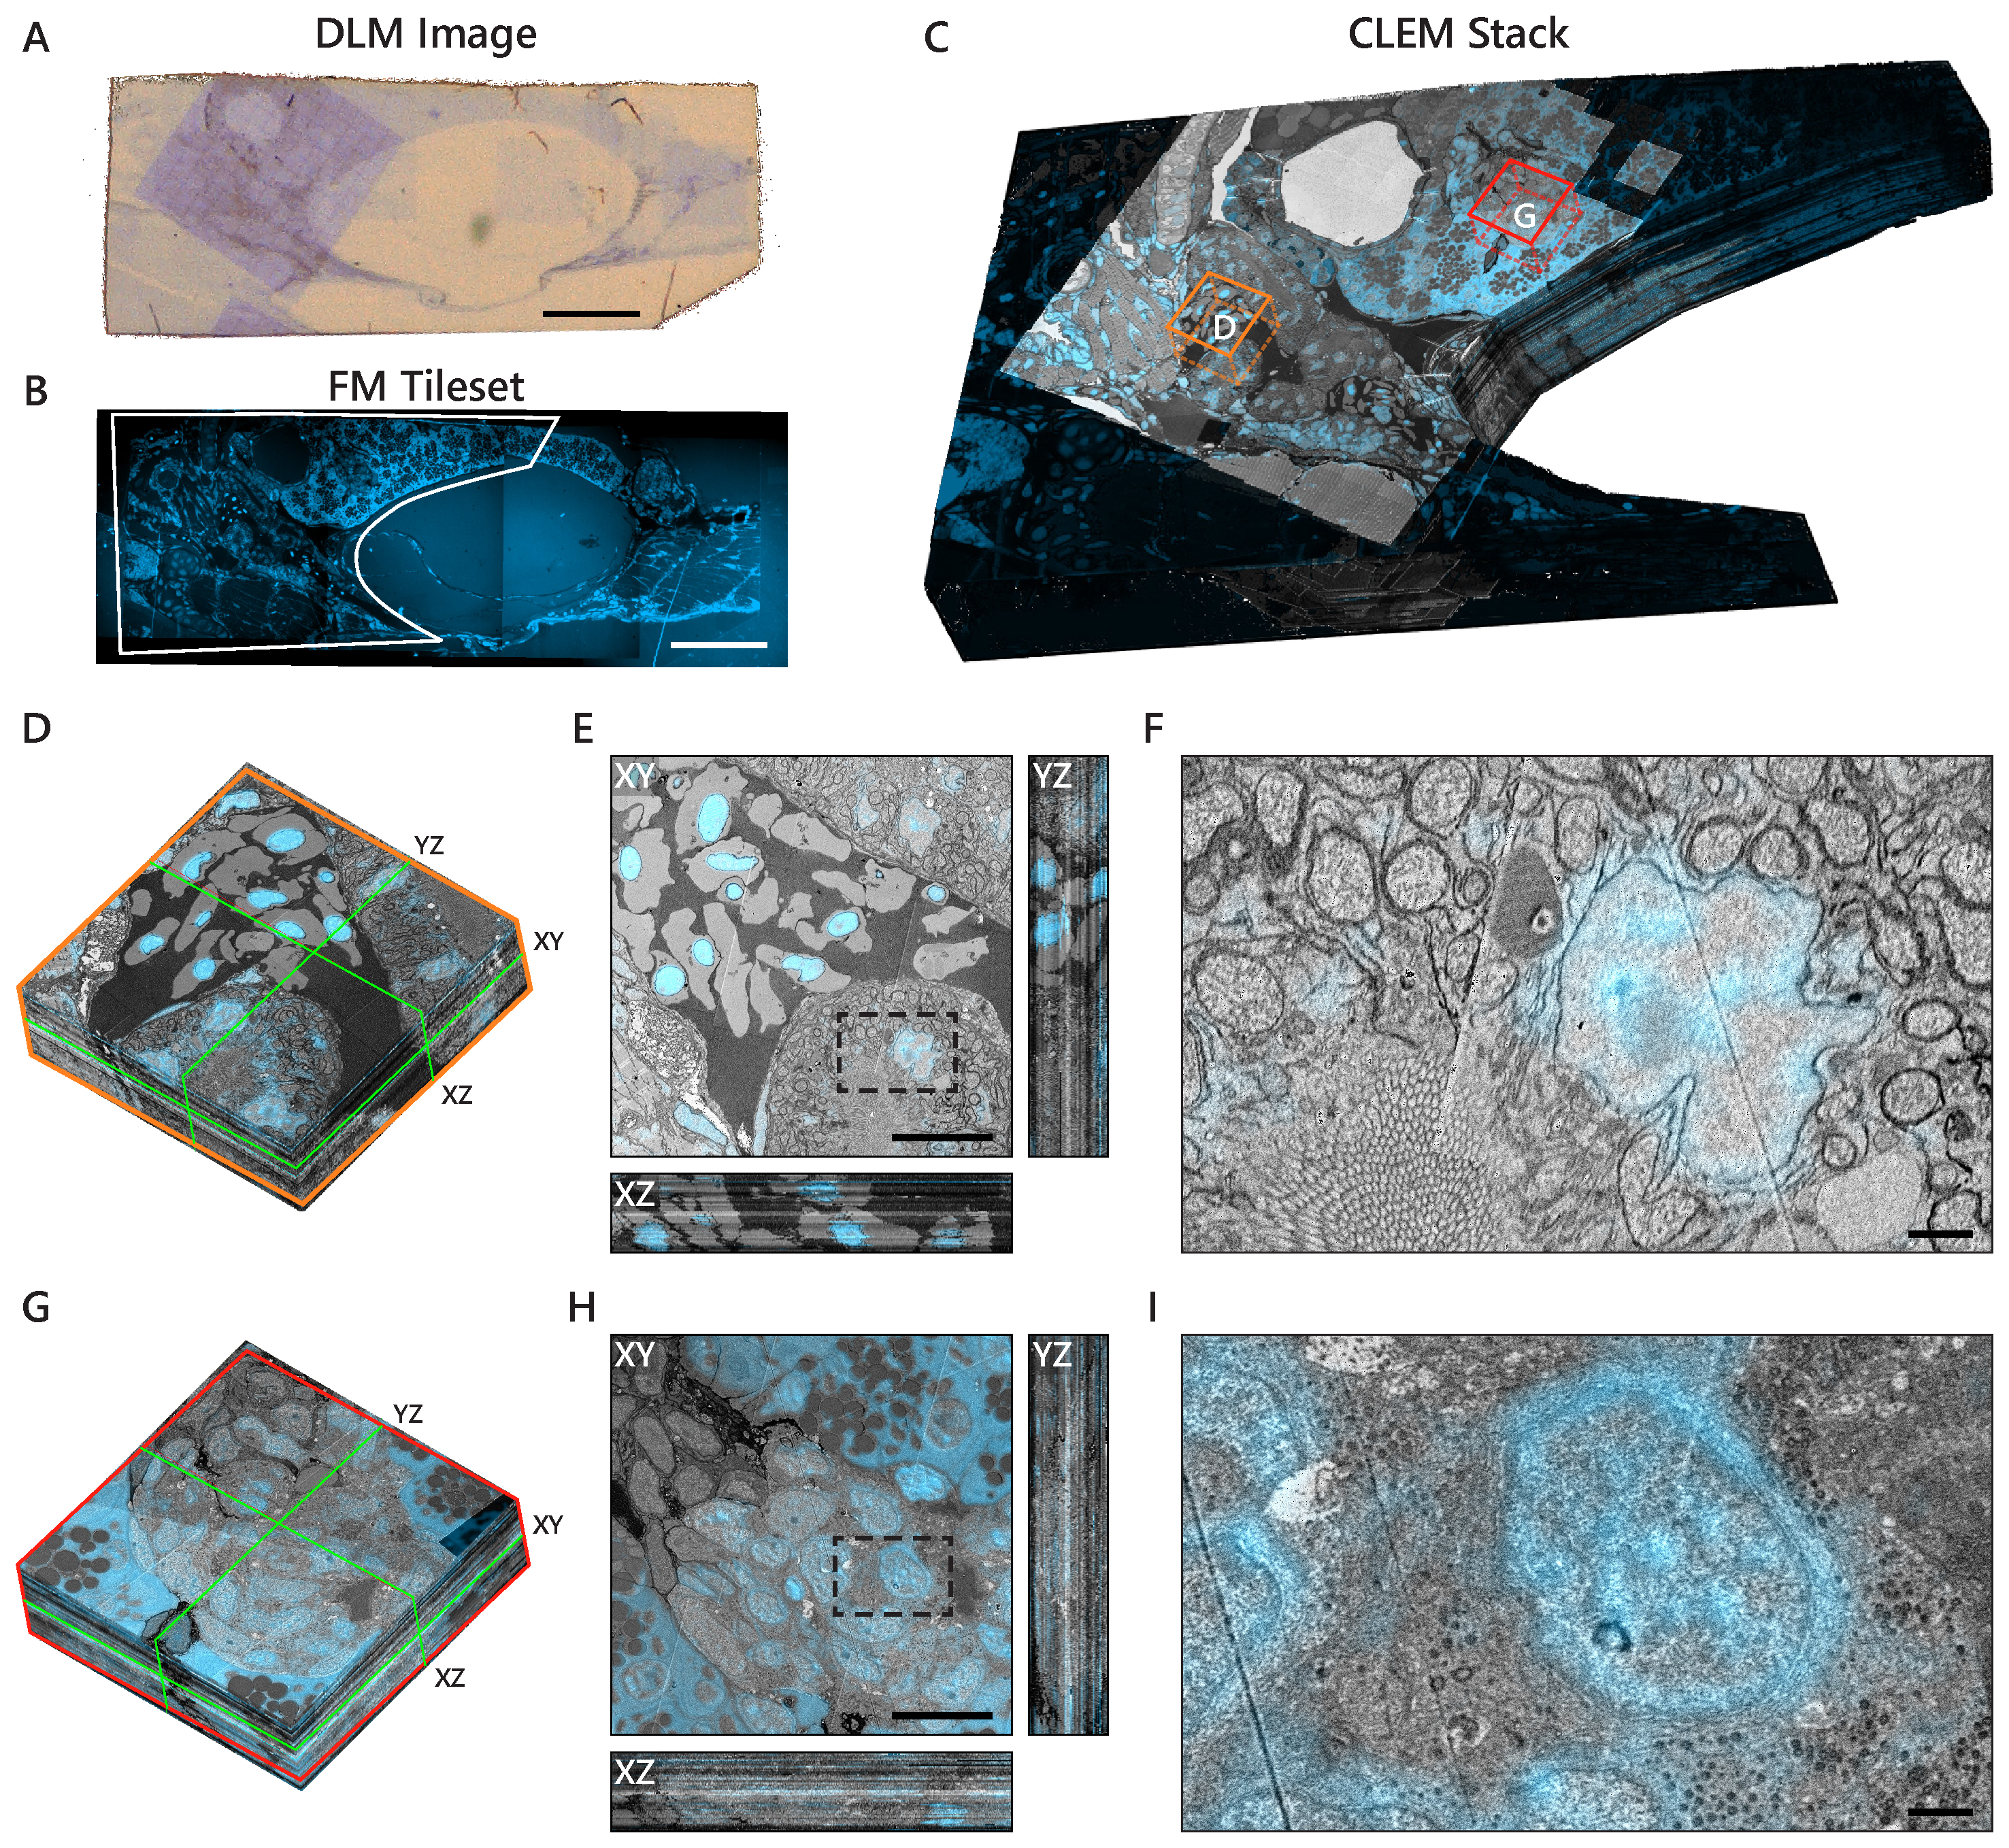
\includegraphics[width=\linewidth]{chapter-3/figures_JPEG_LQ/fig3-6_zebrafish.jpg}
    \caption{Integrated correlative array tomography applied to 63 serial sections of zebrafish pancreas.
    (A) Contrast-enhanced optical image of an individual serial section obtained by the DLM. The section was re-acquired post-EM imaging, revealing the region of interest irradiated by the electron beam. The biological material can be seen in pale blue in contrast with the bare EPON (brown background).
    (B) Hoechst signal of an individual serial section, outlining (white) the portion of the tissue shown in (C).
    (C) CLEM volume of the zebrafish tissue cropped to the ROI selected for high-magnification EM imaging—plus a portion of the surrounding fluorescence signal. Sub-stacks for inspection are denoted by orange (D\,--\,F) and red (G\,--\,I) boxes.
    (D) 3D sub-stack of muscle tissue within the zebrafish pancreas. Green lines indicate orthoslices of the $XY$, $XZ$, and $YZ$ planes shown in (E).
    (F) Zoomed-in region of the $XY$ plane showing high-precision FM overlay of Hoechst onto a cell nucleus. (G\,--\,I) Same as in (D\,--\,F), but for an islet of Langerhans. Ill-defined cell and organelle membranes in (H) and (I) indicate suboptimal preservation of the ultrastructure in this region of the pancreas.
    Scale bars: (A, B) \SI{100}{\micro\meter}; (E, H) \SI{10}{\micro\meter}; (F, I) \SI{1}{\micro\meter}.
    Raw data at full resolution is available via Nanotomy.}
    \label{fig:3.6_zfpancreas}
\end{figure}

We generally observe high EM-FM overlay precision as evidenced by the Hoechst signal confined to the nuclear envelope in the muscle tissue (Figure \ref{fig:3.6_zfpancreas}E, F). The registration accuracy does, however, exhibit variability in several sections---more so than is seen in the rat pancreas tissue where it appears limited to the gaps between low-magnification EM tiles. In these instances, the inaccuracy stems from a malfunction in the CL registration procedure itself (Supplementary Figure \ref{fig:3.S1_misalignment}G\,--\,N). Variations in the EM image intensity, particularly in the islet, can also be observed for a number of sections (Figure \ref{fig:3.6_zfpancreas}H: $XZ$ and $YZ$ cross-sections). We attribute these artifacts primarily to ultrastructure preservation as they do not appear to be as prevalent in the muscle tissue. While the SEM imaging parameters and detection settings were held constant throughout the acquisition, day-to-day changes in the environment (e.g. temperature, humidity levels) may have varied.

In total, 66 sections were prepared, of which three ($z = \text{9, 10, 34}$) were discarded due to excess surface debris. The omission of consecutive sections was mitigated by extending the SIFT feature depth search from 2 to 3 such that sections $z = \text{8}$ and $z = \text{11}$ could be registered. Total acquisition times for low-magnification CLEM and high-magnification EM were \SI{7.2}{\hour} and \SI{71}{\hour} respectively, versus \SI{335}{\hour} for full section imaging at high-magnification.
